\section{System Design and Architecture}

\subsection{Overview of the System}
The following figure shows an overview of the system architecture of FlowX.
Refer to each microservice's section for more details on the implementation.

\begin{figure}[H]
    \centering
    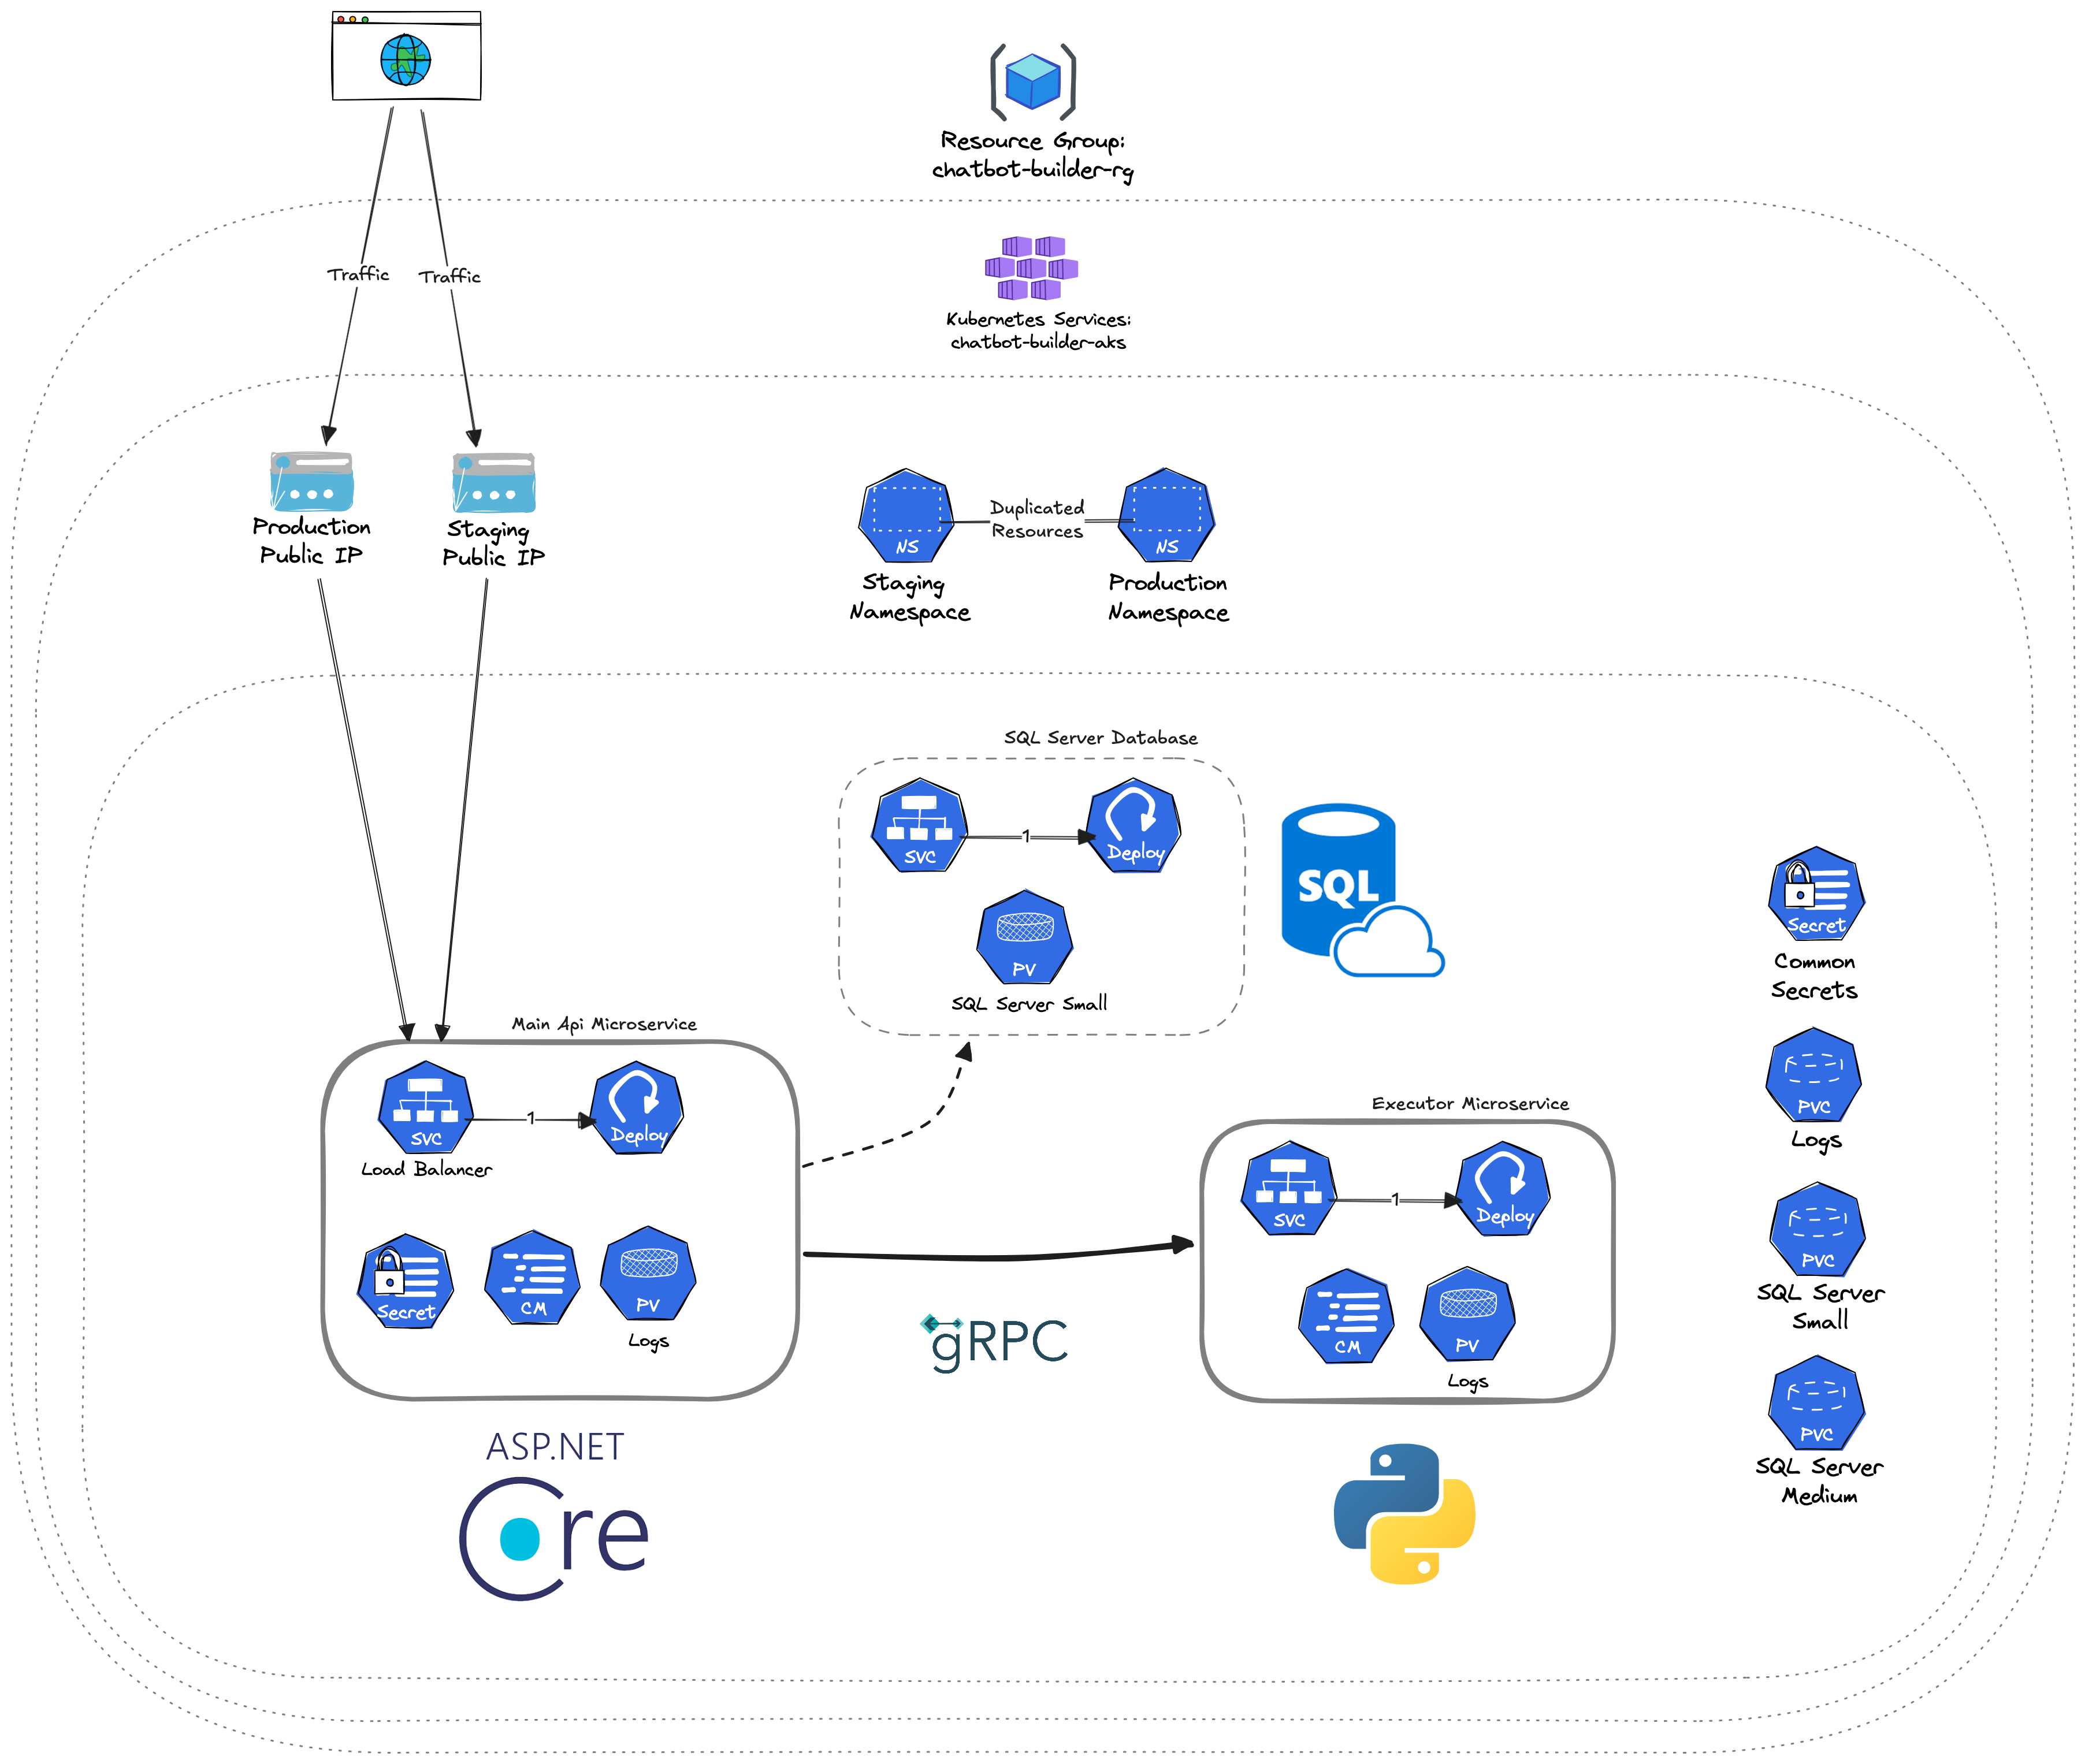
\includegraphics[width=0.95\textwidth]{assets/SystemDesign.png}
    \caption{Microservices architecture of FlowX}
    \label{fig:system_design}
\end{figure}

The project was developed using a microservices architecture, with separate repositories for each microservice and the frontend client. The repositories are as follows:
\begin{itemize}
    \item \textbf{chatbot-builder-api}: The main API microservice for the Chatbot Builder application. Responsible for authentication and orchestrating workflows traversal \& state-management, uses the Executor-Service for LangChain logic.
    \item \textbf{chatbot-builder-executor}: The LangChain execution microservice for the Chatbot Builder application. Controlled by the API-Service, responsible for executing LangChain logic in workflows.
    \item \textbf{chatbot-builder-infra}: Infrastructure \& deployment of the Chatbot Builder application using Terraform \& Kubernetes.
    \item \textbf{chatbot-builder-client}: The frontend for the Chatbot Builder application, built with React Native.
    \item \textbf{chatbot-builder-protos}: Protocol Buffers schema definitions for gRPC communication between API and Executor services.
\end{itemize}

\subsection{API Microservice}
This is the main API microservice for the Chatbot Builder application. It is responsible for authentication and orchestrating workflows traversal \& state-management.

Implemented using ASP.NET Core, which provides a robust strongly typed framework that is easy to maintain and scale.

The following is a few of the key features of the API microservice:
\begin{itemize}
    \item Authentication: JWT-based authentication for user management.
    \item Workflow Management: CRUD operations for workflows, nodes, and connections.
\end{itemize}

\subsection{Executor Microservice}
This is the LangChain execution microservice for the Chatbot Builder application. It is controlled by the API-Service and is responsible for executing LangChain logic in workflows.

Implemented using Python, which contains the Langchain library that abstracts LLM model management and execution.

The following is a few of the key features of the Executor microservice:
\begin{itemize}
    \item gRPC Service: Allows for calls from the API service to execute LangChain logic.
\end{itemize}